\documentclass[11pt,letterpaper]{article}

% ---- packages ----
\usepackage[margin=0.9in]{geometry}
\usepackage{graphicx}
\usepackage{booktabs}
\usepackage{hyperref}
\usepackage{amsmath}
\usepackage{xcolor}
\usepackage{float}
\usepackage{enumitem}
\usepackage[T1]{fontenc}
\usepackage{lmodern}

\hypersetup{colorlinks=true, linkcolor=blue!60!black, citecolor=blue!60!black, urlcolor=blue!60!black}
\setlength{\parindent}{0pt}
\setlength{\parskip}{6pt}

\title{\textbf{Research Question 3: Unsupervised Accident Clustering\\on Long Island}}
\author{
Shane Patandin \quad Matthew Tranquada \quad Vraj Patel\\
Kaushal Patel \quad Sur Vaghasiya\\[4pt]
\textit{AMS 597 --- Statistical Machine Learning}\\
\textit{Stony Brook University \textperiodcentered{} Spring 2025}
}
\date{}

\begin{document}
\maketitle
\thispagestyle{empty}

%======================================================================
\section{Research Question}
%======================================================================

\emph{Discover patterns in accidents by grouping similar incidents based on weather and road characteristics using clustering techniques in R.}

We operationalise this question through two complementary clustering tracks---\emph{scenario clustering} (what type of accident?) and \emph{spatial clustering} (where does it concentrate?)---then cross-tabulate the results to identify which accident profiles dominate each highway corridor. Specifically, we ask whether unsupervised learning can reveal distinct accident archetypes on Long Island, and whether those archetypes differ meaningfully in severity risk.
Cluster quality is assessed with silhouette width and bootstrap stability; cluster drivers are decoded with a Random Forest SHAP bridge.

%======================================================================
\section{Data \& Preprocessing}
%======================================================================

\subsection{Dataset}

The dataset is a cleaned subset of US Accidents (March 2023 release) filtered to Nassau and Suffolk counties via ZIP-code boxing (110xx, 115xx, 117xx--119xx). After removing 147 western-edge Queens records, the final dataset contains \textbf{33,228 accidents} across 48 raw columns spanning March 2016--March 2023.

\subsection{Feature Engineering}

Phase~3 of the pipeline derives all analysis-ready features from raw columns. The key transformations are summarised below.

\begin{table}[H]
\centering
\small
\caption{Engineered features for scenario clustering.}
\begin{tabular}{@{}llp{6.5cm}@{}}
\toprule
\textbf{Domain} & \textbf{Features} & \textbf{Notes} \\
\midrule
Temporal (factor) & hour\_band, rush\_hour, Sunrise\_Sunset, weekday, weekend, season & 6-level hour band; rush = 6--9 AM / 3--6 PM \\
Weather (factor) & weather\_group (7 levels) & 37 raw labels collapsed to Clear, Cloudy, Rain, Snow/Ice, Fog/Haze, Thunderstorm, Other \\
Infrastructure & Junction, Crossing, Traffic\_Signal, Stop & Boolean flags retained after zero-variance audit \\
Weather (numeric) & Temperature(F), Humidity(\%), Visibility(mi), Pressure(in), Wind\_Speed(mph) & Median-imputed where missing ($<$1\%) \\
Duration & log\_Duration & 99th-percentile-capped, then log1p transformed \\
\bottomrule
\end{tabular}
\end{table}

\textbf{Design principle:} Severity is intentionally excluded from all clustering inputs. It is used only afterward for post-cluster profiling, so that cluster discovery is driven by pre-accident observable conditions, not by outcome.

%======================================================================
\section{Methods}
%======================================================================

\subsection{Pipeline Architecture}

The workflow operates on two independent tracks that merge at Phase~8 for joint interpretation.

\begin{enumerate}[nosep]
\item \textbf{Scenario track} (Phases 5--6): discovers accident \emph{types} based on weather, time-of-day, season, and infrastructure features.
\item \textbf{Spatial track} (Phase 7): discovers geographic \emph{hotspot corridors} based on projected latitude/longitude.
\item \textbf{Integration} (Phase 8): joins both label sets onto every record; profiles clusters by severity, county, weather, and time.
\item \textbf{Explainability} (Phase 8B): trains a 500-tree Random Forest to predict cluster membership, then extracts permutation importance and Shapley values to explain what drives each cluster.
\end{enumerate}

\subsection{Scenario Clustering: k-Prototypes (Baseline)}

k-Prototypes extends k-Means to mixed data by combining squared Euclidean distance for continuous variables with simple matching distance for categorical variables. We fit candidates at $k \in \{3, \ldots, 8\}$ with \texttt{type="gower"} range-normalisation, \texttt{nstart=10}, and seed~42.

This baseline produced a best silhouette of \textbf{0.1616} at $k=3$, well below the 0.30 acceptance threshold (Kaufman \& Rousseeuw, 1990), with a Jaccard bootstrap stability of \textbf{0.243}---far below the 0.60 acceptable level (Hennig, 2007). The quality gate classified all findings as \textsc{exploratory}.

\subsection{Scenario Clustering: FAMD + k-Means (Enhanced)}

To improve cluster separation, we implemented a two-stage dimensionality reduction strategy guided by SHAP feature importance.

\textbf{Step 1: Feature selection.} The Phase~8B SHAP analysis ranked all 17 scenario features by permutation importance (Table~\ref{tab:importance}). The bottom 9 features---weekday, log\_Duration, weekend, Wind\_Speed, Pressure, Crossing, Traffic\_Signal, Junction, Stop---all had near-zero importance scores. Retaining them contributes to the curse of dimensionality without aiding separation, so they were dropped. The top 8 features were retained: rush\_hour, hour\_band, Sunrise\_Sunset, Visibility(mi), weather\_group, Humidity(\%), Temperature(F), and season.

\textbf{Step 2: FAMD transformation.} Factor Analysis of Mixed Data (\texttt{FactoMineR::FAMD}) projects the 8 mixed-type features into orthogonal numeric components. FAMD handles categorical variables via indicator expansion with appropriate scaling, producing real-valued axes on which Euclidean distance is geometrically meaningful.

\textbf{Step 3: Component selection.} A grid search over 20 (ncomp $\times$ k) combinations evaluated silhouette width for each setting. The results are unambiguous: \textbf{4 components with $k=4$} yields the highest silhouette at 0.4268. Retaining additional components degrades separation monotonically---from 0.43 (4 components) to 0.25 (7 components)---because the tail components capture noise rather than structure.

\textbf{Step 4: k-Means clustering} on the 4-dimensional FAMD coordinate matrix, with \texttt{nstart=25} and \texttt{iter.max=100}.

\subsection{Spatial Clustering: DBSCAN}

DBSCAN operates on km-projected coordinates ($x_\text{km}$, $y_\text{km}$) computed from a local tangent-plane projection anchored at $(40.8^\circ\text{N},\, 73.2^\circ\text{W})$. A 68-combination grid search over $\text{eps} \in [0.3, 2.0]$\,km and $\text{minPts} \in \{40, 50, 75, 100\}$ selected eps\,=\,1.0\,km and minPts\,=\,100, satisfying all acceptance criteria: 12 non-noise clusters, 15.3\% noise, largest cluster at 44.1\%.

%======================================================================
\section{Results}
%======================================================================

\subsection{FAMD Eigenvalue Structure}

\begin{table}[H]
\centering
\small
\caption{FAMD eigenvalues for the top 8 mixed-type scenario features.}
\begin{tabular}{@{}cccc@{}}
\toprule
\textbf{Component} & \textbf{Eigenvalue} & \textbf{Variance \%} & \textbf{Cumulative \%} \\
\midrule
1 & 2.574 & 12.87 & 12.87 \\
2 & 2.176 & 10.88 & 23.75 \\
3 & 1.746 & 8.73  & 32.48 \\
\textbf{4 (retained)} & \textbf{1.460} & \textbf{7.30} & \textbf{39.78} \\
5--10 & $<$1.13 each & 5.0--5.6 each & up to 71.36 \\
\bottomrule
\end{tabular}
\end{table}

Four components capture 39.78\% of total variance. While this is below the conventional 80\% retention rule, the grid search confirms that additional components degrade silhouette---a clear case where the bias-variance trade-off favours fewer, cleaner dimensions over maximal variance retention.

\subsection{Method Comparison}

\begin{table}[H]
\centering
\caption{Scenario clustering: k-Prototypes baseline vs.\ FAMD + k-Means.}
\begin{tabular}{@{}lcccc@{}}
\toprule
\textbf{Method} & \textbf{k} & \textbf{Silhouette} & \textbf{Stability} & \textbf{Selected} \\
\midrule
k-Prototypes (Gower) & 3 & 0.1616 & 0.243 (Jaccard) & No \\
\textbf{FAMD + k-Means (Euclidean)} & \textbf{4} & \textbf{0.4268} & \textbf{0.997 (ARI)} & \textbf{Yes} \\
\bottomrule
\end{tabular}
\end{table}

The FAMD pipeline improves silhouette by 165\% (0.16 $\to$ 0.43) and produces near-perfect bootstrap reproducibility (ARI\,=\,0.997 over 20 resamples). The quality gate upgrades from \textsc{exploratory} to \textsc{acceptable}.

\subsection{Silhouette by $k$}

\begin{figure}[H]
\centering
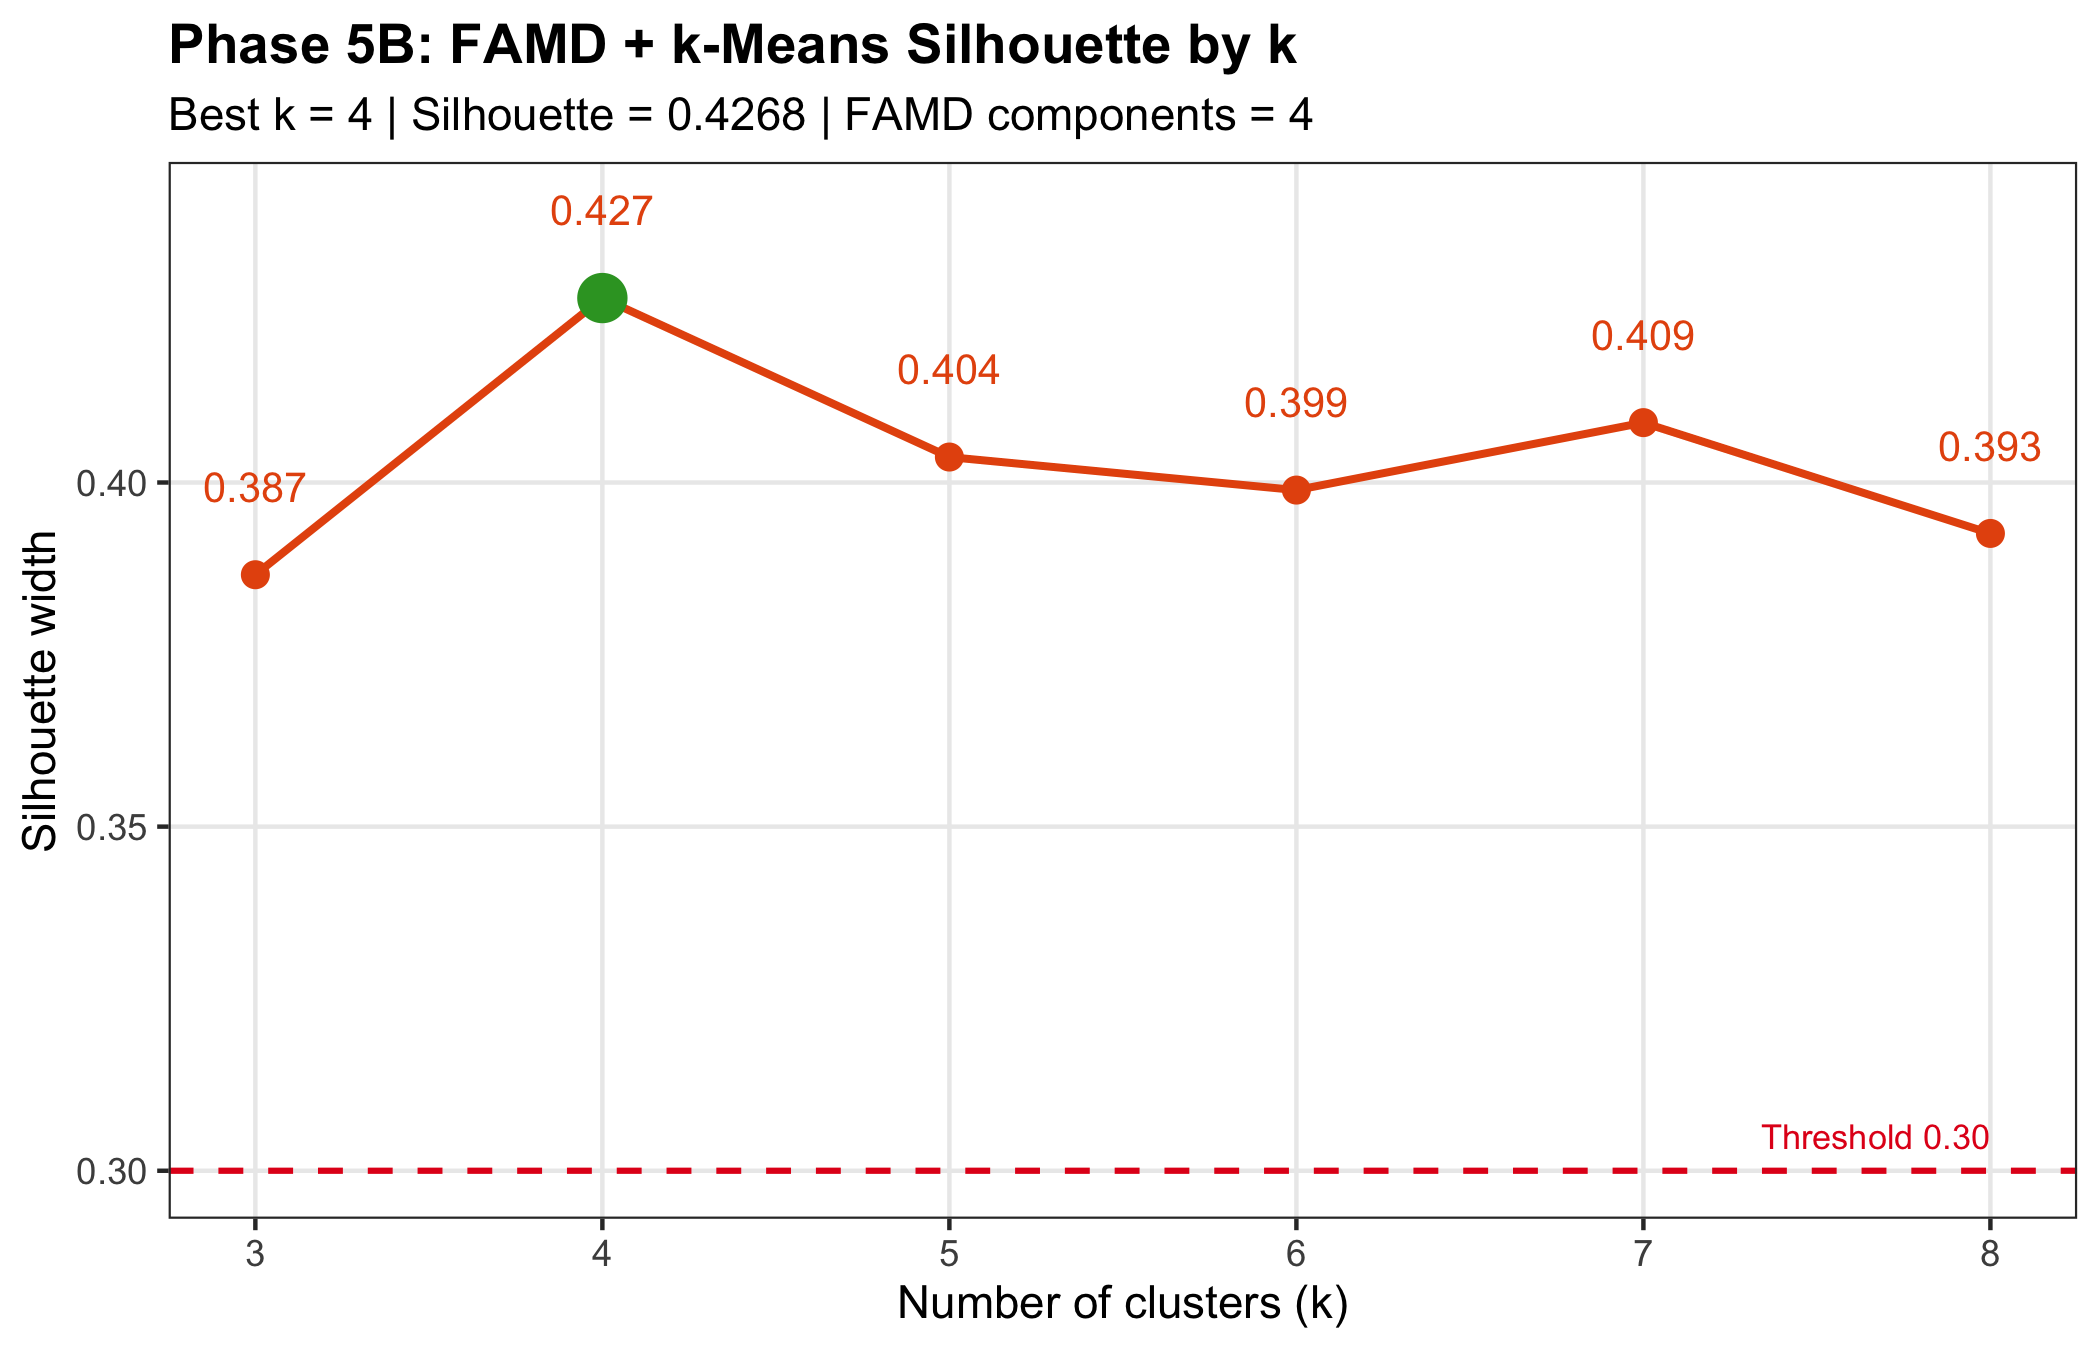
\includegraphics[width=0.65\textwidth]{figures/phase5b_famd_silhouette_plot.png}
\caption{FAMD + k-Means silhouette width by $k$. All candidates clear the 0.30 threshold; $k=4$ achieves the highest score (0.4268).}
\label{fig:sil}
\end{figure}

\subsection{FAMD Biplot}

\begin{figure}[H]
\centering
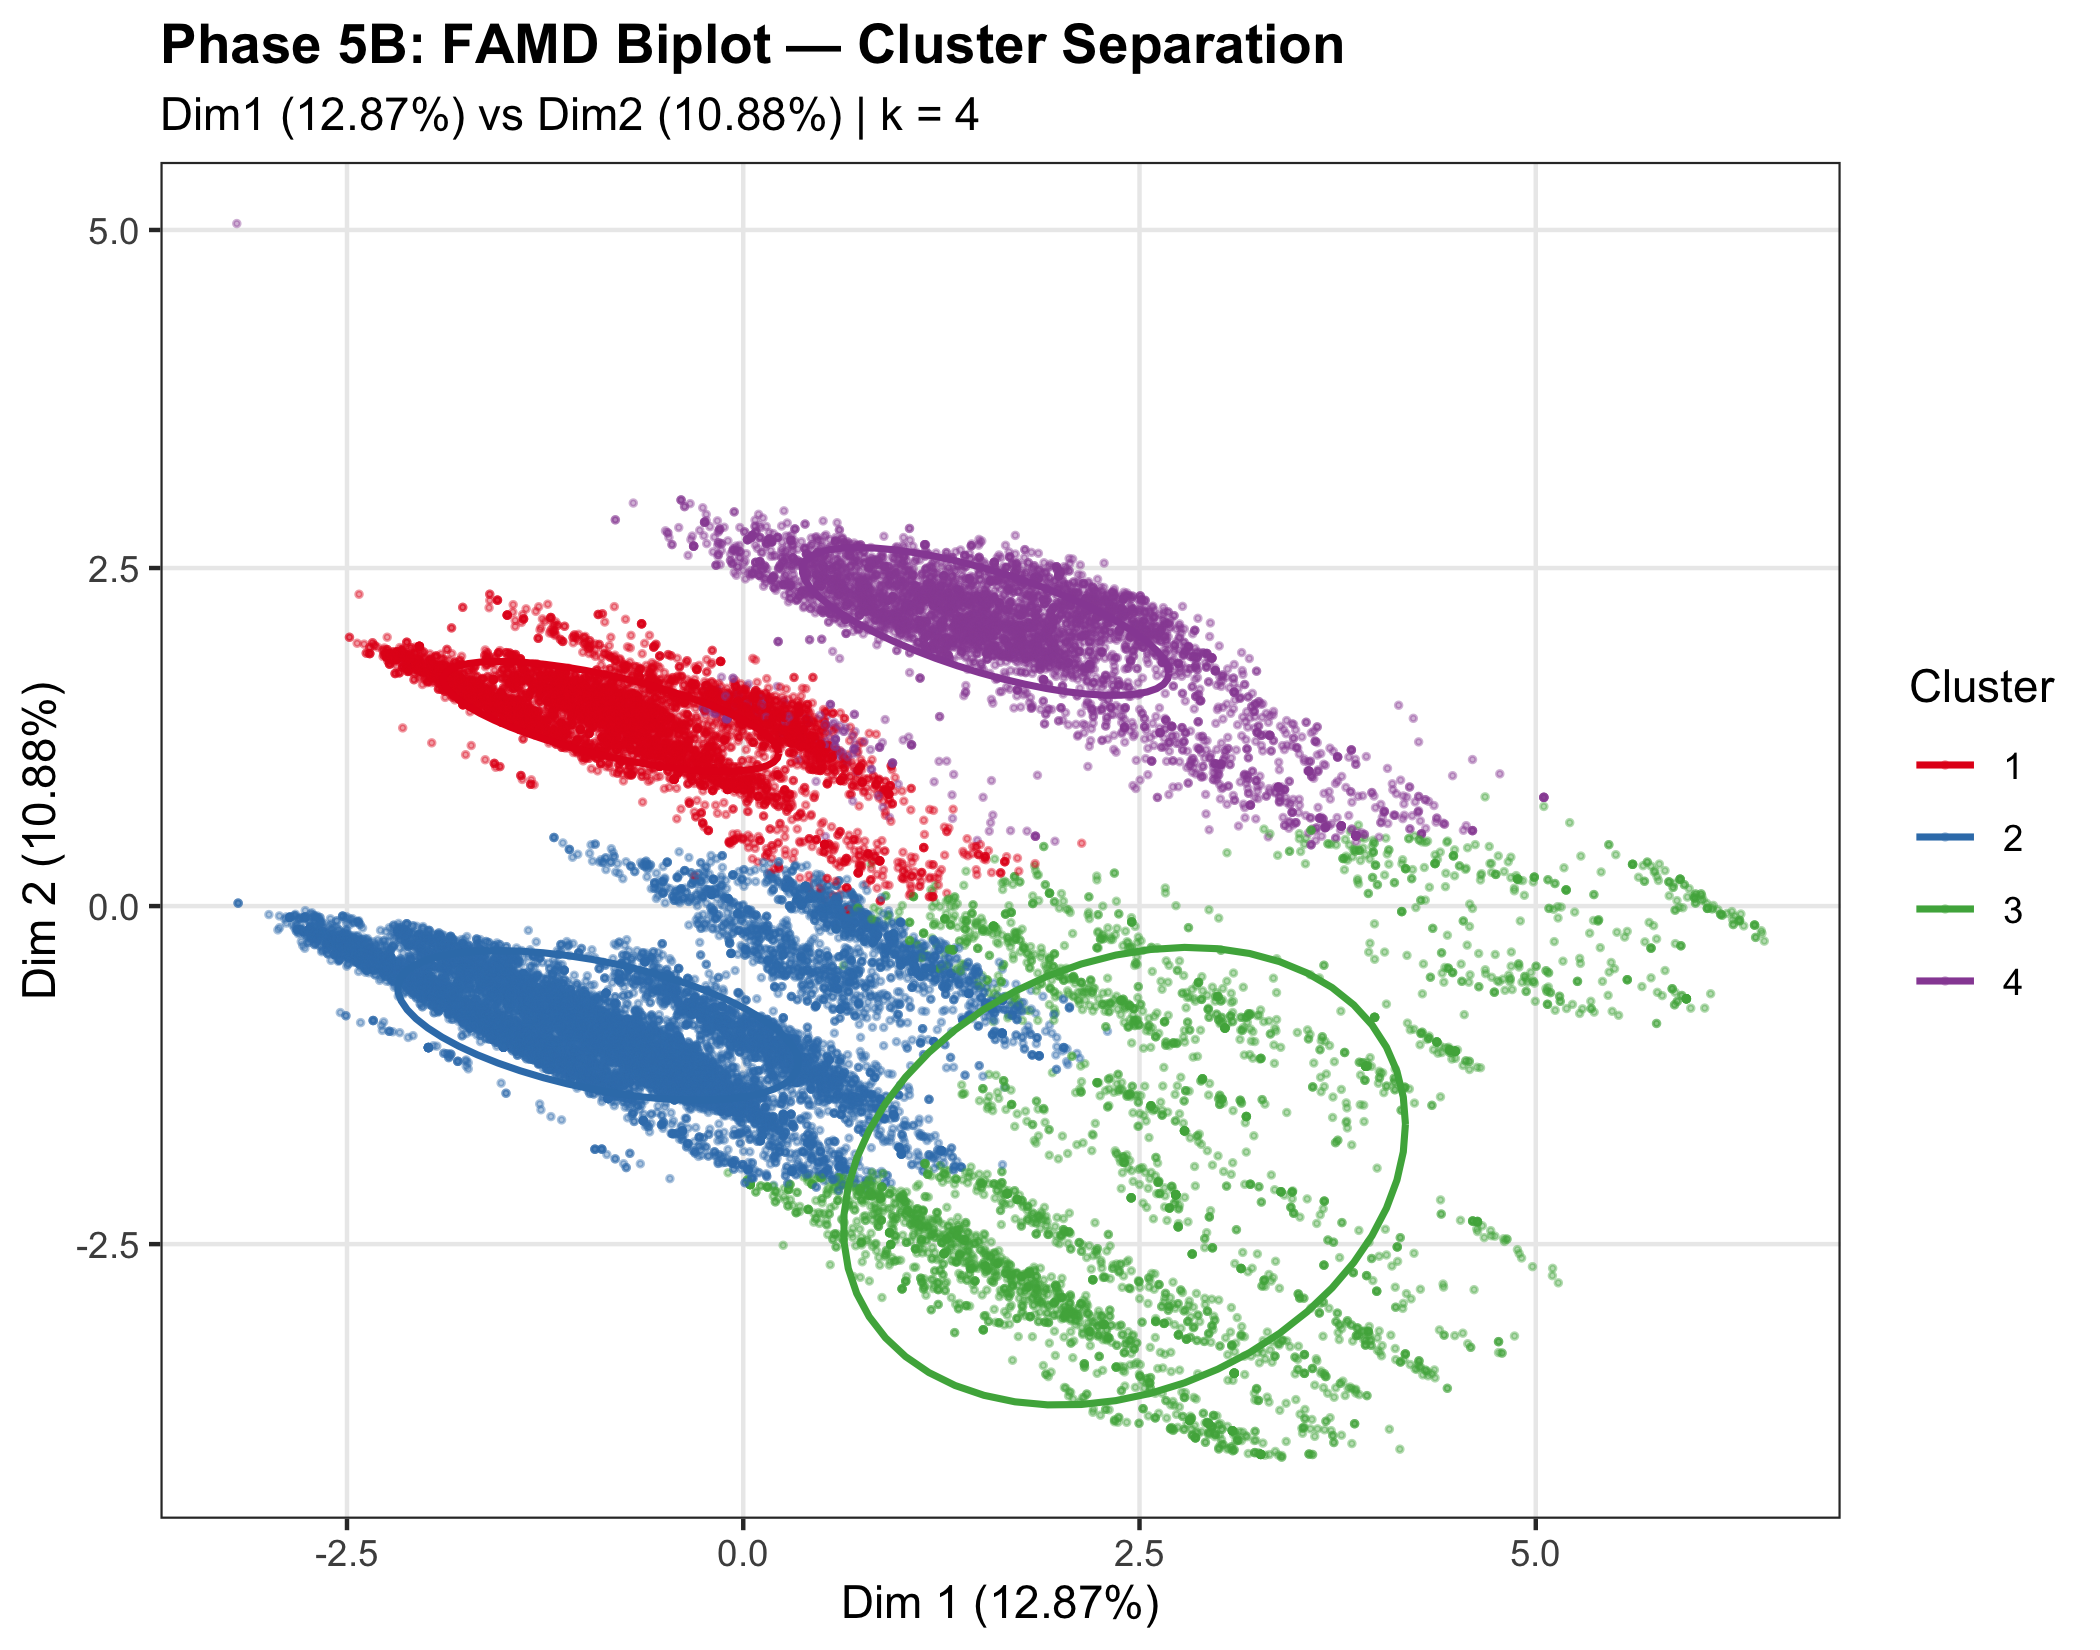
\includegraphics[width=0.65\textwidth]{figures/phase5b_famd_biplot.png}
\caption{FAMD biplot (Dim~1 vs.\ Dim~2) coloured by cluster assignment ($k=4$). The 68\% concentration ellipses show meaningful geometric separation between clusters.}
\label{fig:biplot}
\end{figure}

\subsection{The Four Accident Archetypes}

\begin{table}[H]
\centering
\small
\caption{Scenario cluster profiles---the four discovered accident archetypes.}
\label{tab:profiles}
\begin{tabular}{@{}clccccp{3cm}c@{}}
\toprule
\textbf{C} & \textbf{Name} & \textbf{Size} & \textbf{Sev4\%} & \textbf{Night\%} & \textbf{Wknd\%} & \textbf{Dominant conditions} & \textbf{Risk} \\
\midrule
1 & Cloudy Off-Peak & 7,220 & 2.9 & 0 & 19 & Cloudy, Midday, 64\textdegree F, vis 9.9\,mi & Baseline \\
2 & AM Rush & 16,754 & 1.8 & 13 & 10 & Cloudy, AM Rush, Junction-heavy & Low \\
3 & Rain AM Rush & 3,730 & 2.1 & 23 & 12 & Rain (51\%), vis 3.1\,mi & Baseline \\
\textbf{4} & \textbf{Night / Early AM} & \textbf{5,524} & \textbf{6.1} & \textbf{97} & \textbf{29} & Cloudy, 53\textdegree F, vis 9.5\,mi & \textbf{High} \\
\bottomrule
\end{tabular}
\end{table}

\textbf{Cluster~4---Night / Early~AM (High Risk):} 6.1\% Severity~4 rate, which is 2.21$\times$ the dataset baseline of 2.76\%. Nearly all accidents (97\%) occur at night, and the weekend share (29\%) is the highest of any cluster. This is the strongest risk signal in the data and a primary candidate for targeted nighttime safety interventions.

\subsection{SHAP Feature Importance (Phase 8B)}

\begin{figure}[H]
\centering
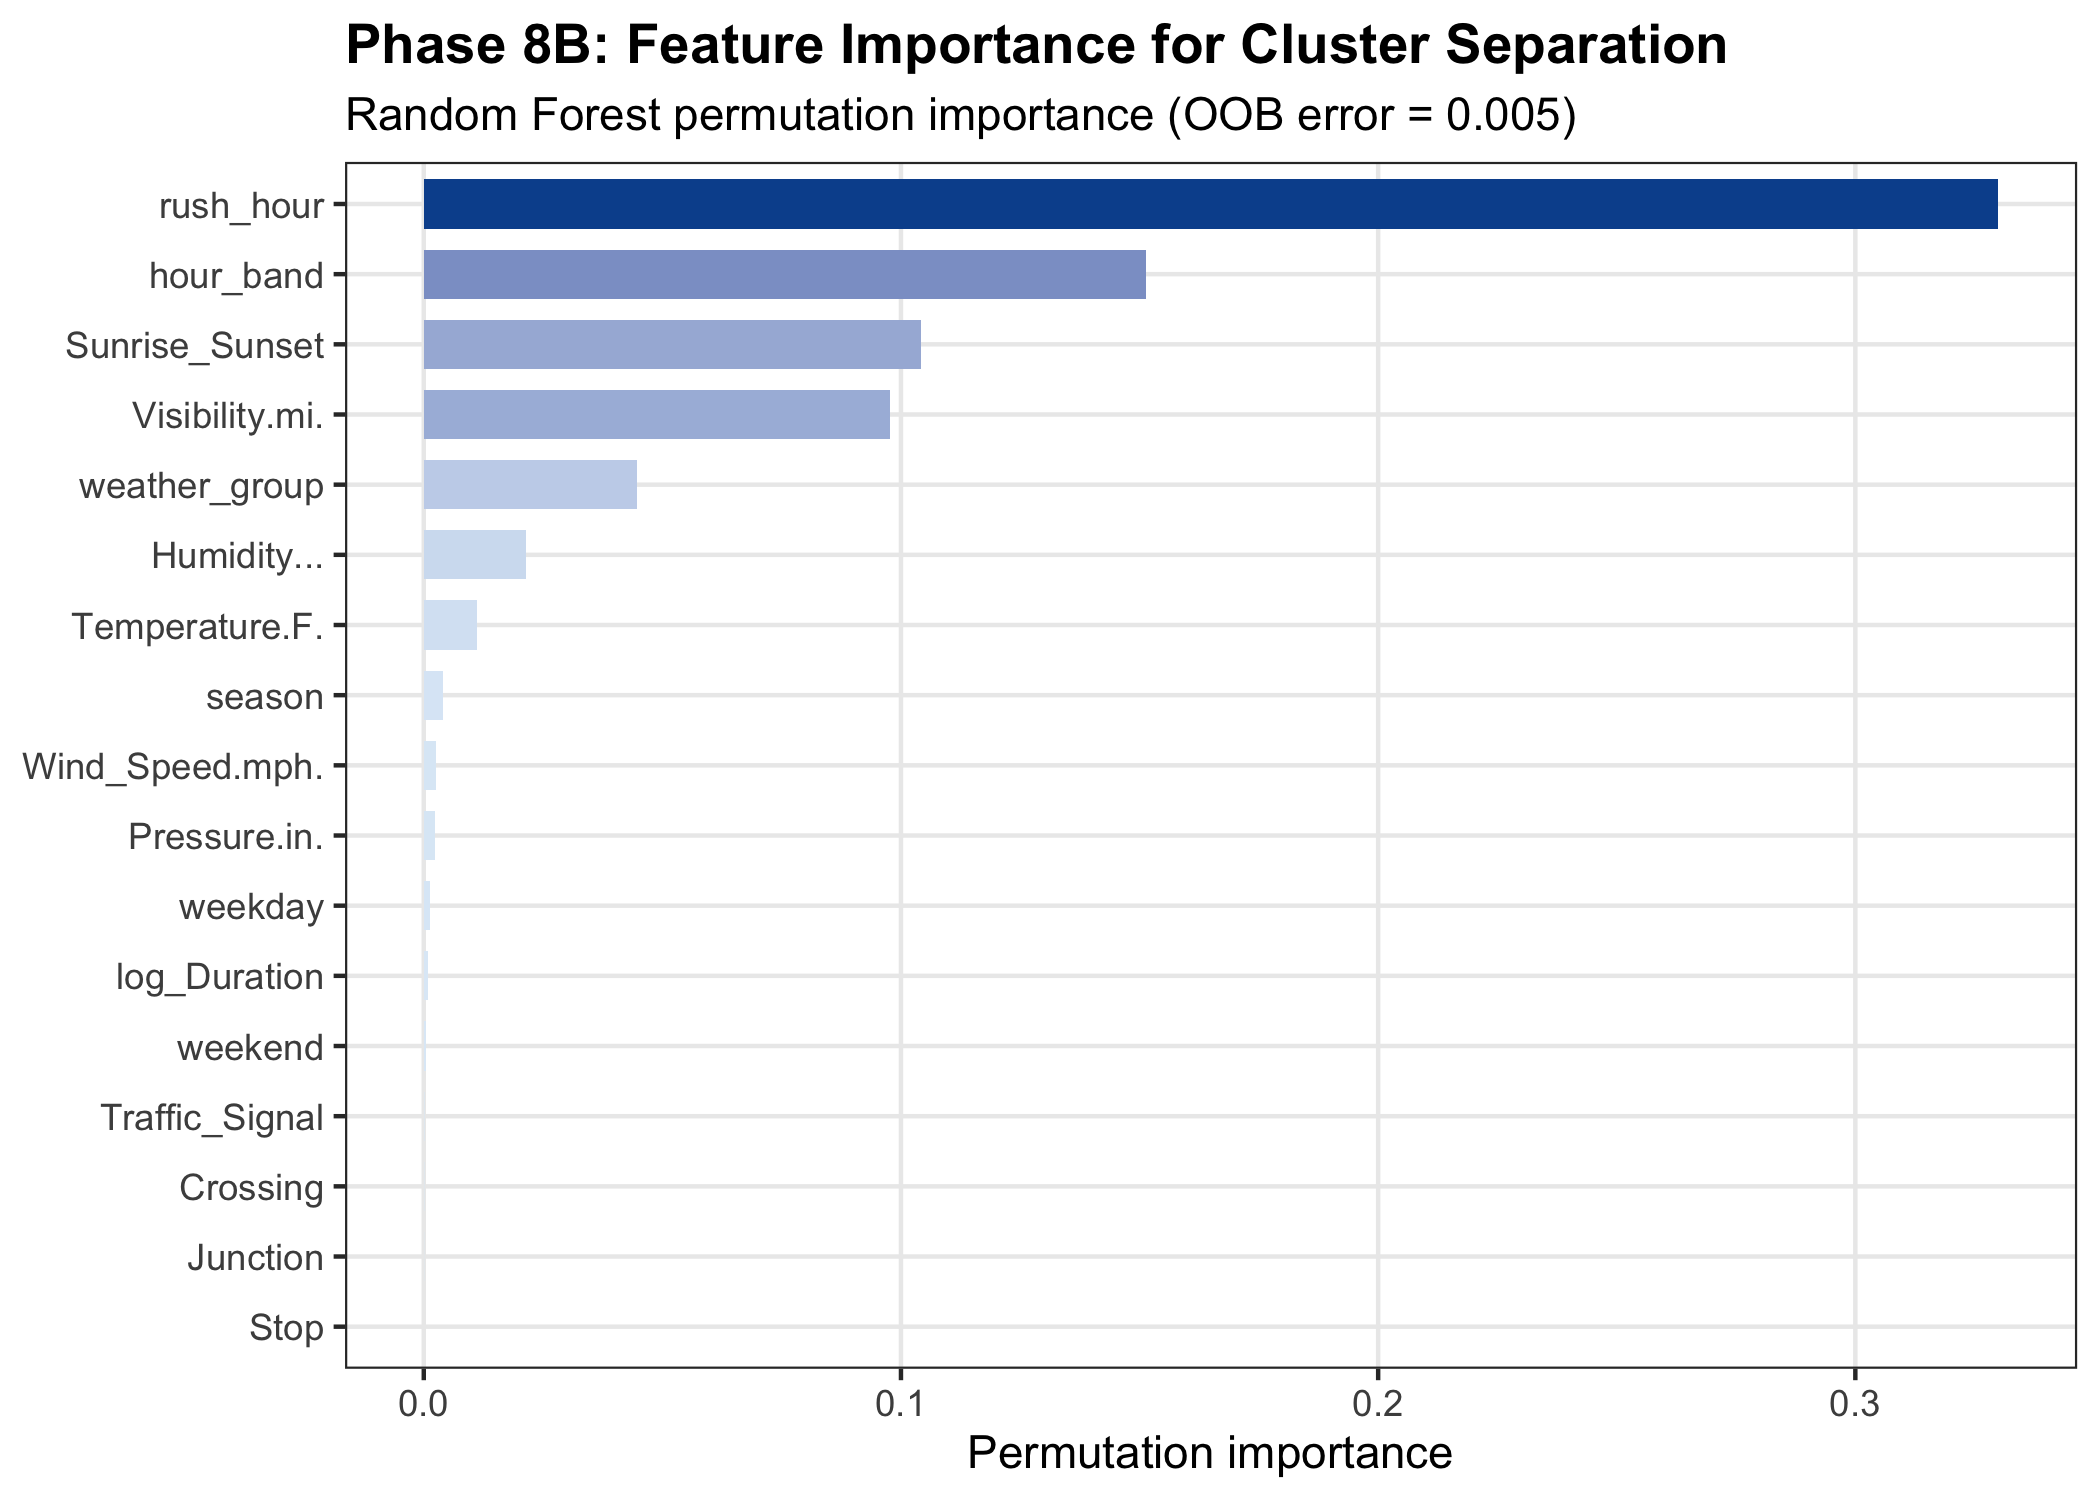
\includegraphics[width=0.60\textwidth]{figures/phase8b_global_importance.png}
\caption{Global permutation importance from a 500-tree Random Forest trained to predict cluster membership (OOB accuracy = 99.6\%).}
\label{tab:importance}
\end{figure}

\begin{table}[H]
\centering
\small
\caption{Top-8 features by permutation importance (Random Forest, OOB = 99.6\%).}
\begin{tabular}{@{}clcl@{}}
\toprule
\textbf{Rank} & \textbf{Feature} & \textbf{Importance} & \textbf{Interpretation} \\
\midrule
1 & rush\_hour      & 0.330 & Single strongest separator \\
2 & hour\_band      & 0.151 & Finer time-of-day resolution \\
3 & Sunrise\_Sunset & 0.104 & Day vs.\ night---drives high-risk C4 \\
4 & Visibility(mi) & 0.098 & Separates rain (C3) from clear (C1) \\
5 & weather\_group  & 0.045 & Rain vs.\ Cloudy vs.\ Clear \\
6 & Humidity(\%)    & 0.021 & Moisture conditions \\
7 & Temperature(F)  & 0.011 & Seasonal temperature signal \\
8 & season          & 0.004 & Winter vs.\ summer baseline \\
\bottomrule
\end{tabular}
\end{table}

The takeaway is that \emph{when} you drive matters substantially more than what the weather is. \texttt{rush\_hour} alone accounts for one-third of the Random Forest's classification power, and the top three features are all temporal.

\subsection{Cluster-Specific Feature Importance}

\begin{figure}[H]
\centering
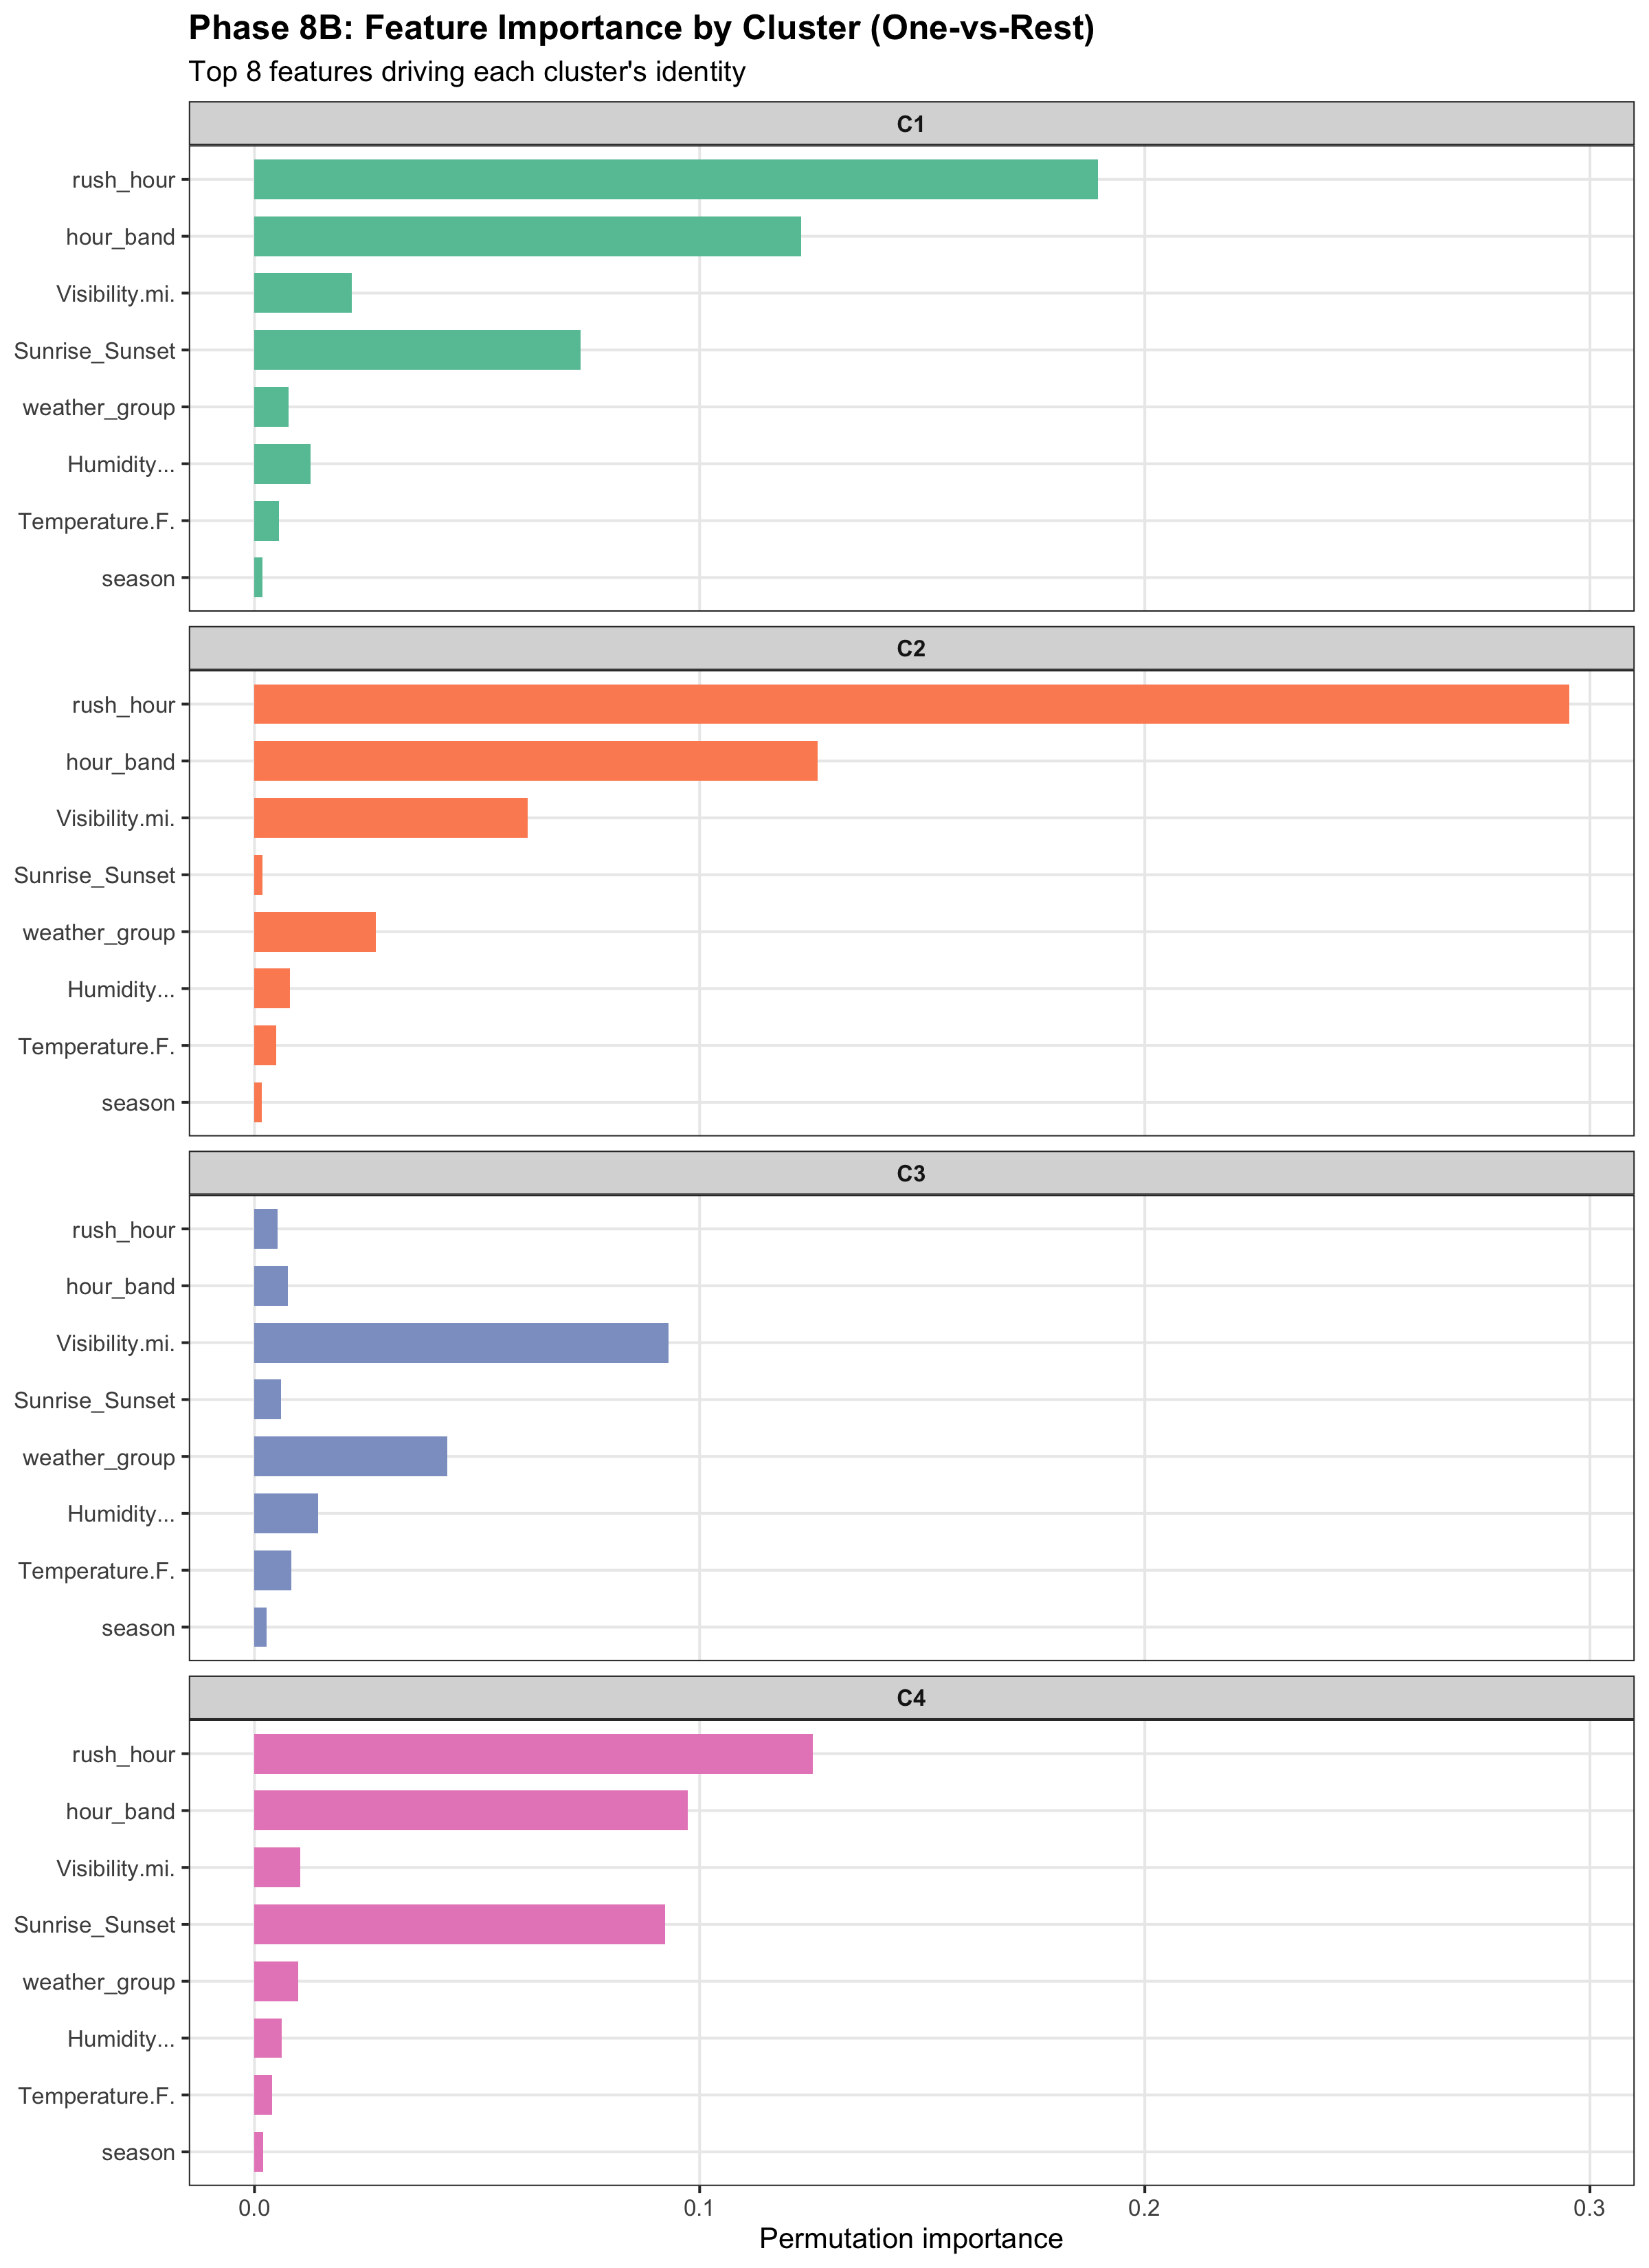
\includegraphics[width=0.68\textwidth]{figures/phase8b_cluster_specific_importance.png}
\caption{Per-cluster Shapley values. Each cluster is characterised by a distinct feature profile, confirming the four archetypes are driven by different combinations of conditions.}
\label{fig:cluster_shap}
\end{figure}

\subsection{Spatial Hotspots (DBSCAN)}

\begin{figure}[H]
\centering
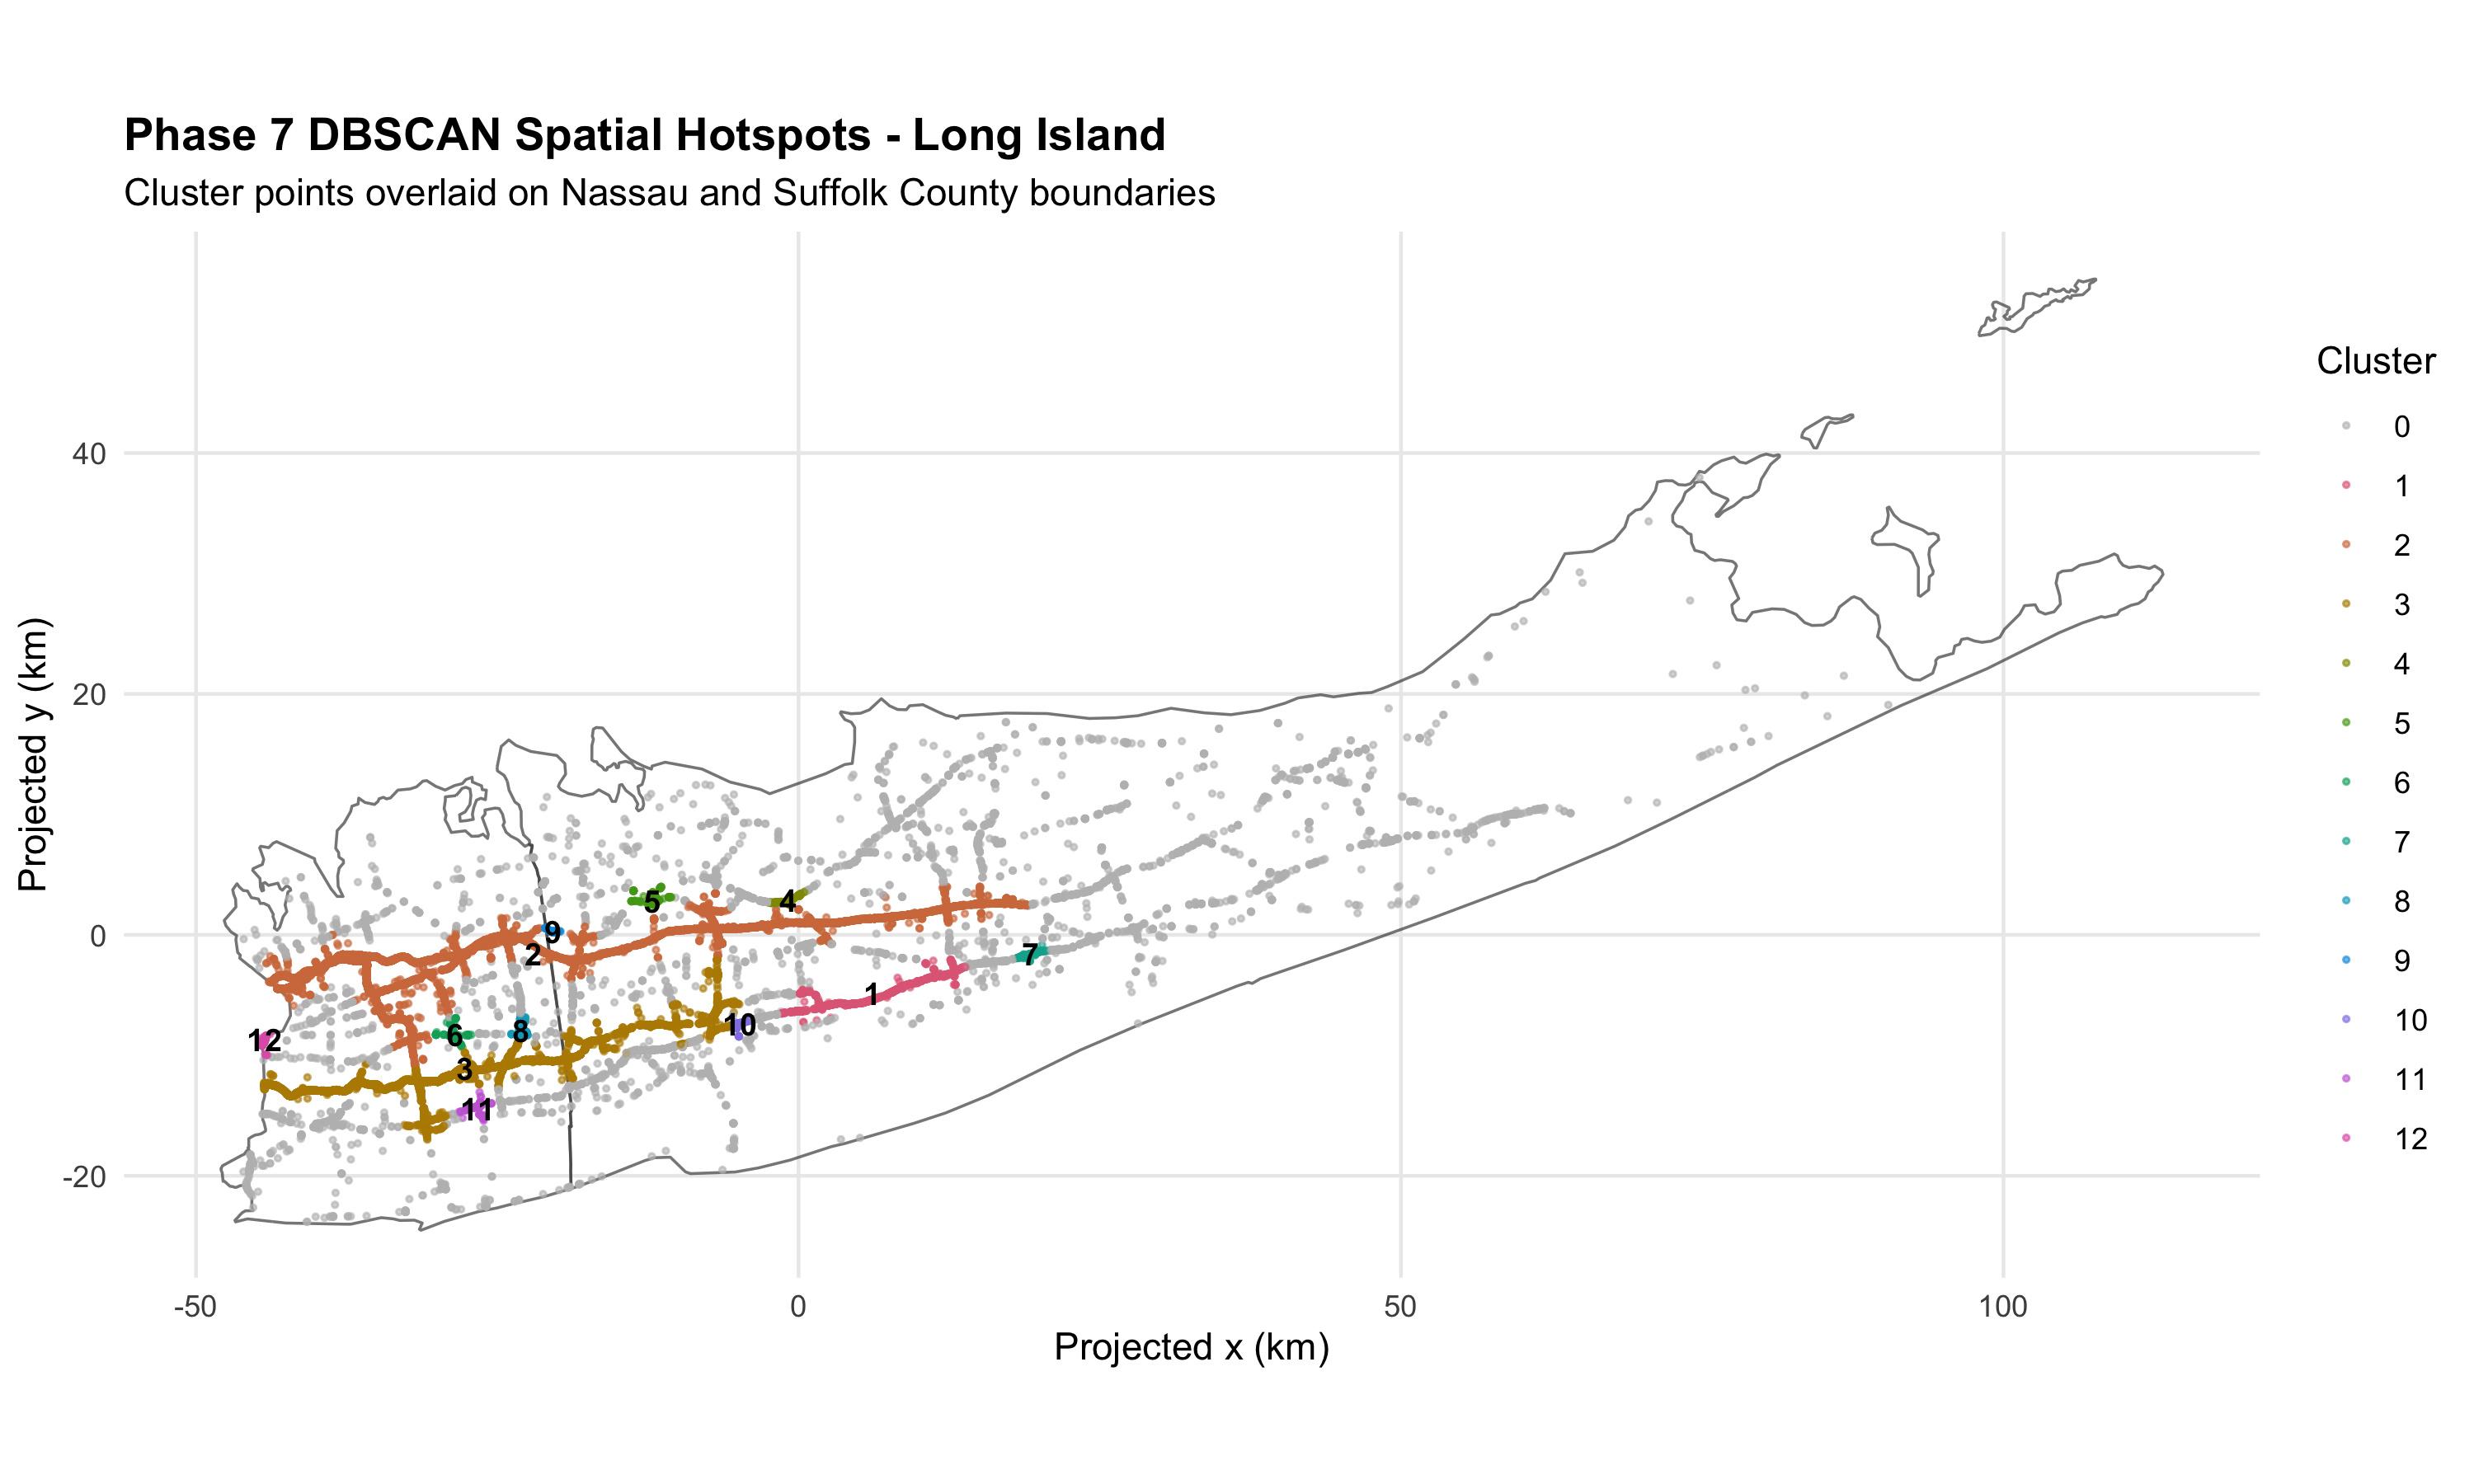
\includegraphics[width=0.65\textwidth]{figures/phase7_spatial_hotspot_map.png}
\caption{DBSCAN spatial clusters (eps\,=\,1.0\,km, minPts\,=\,100). Twelve corridor clusters are identified along Long Island's major east--west highways.}
\label{fig:spatial}
\end{figure}

\begin{table}[H]
\centering
\small
\caption{Top corridor clusters by size.}
\begin{tabular}{@{}clcc@{}}
\toprule
\textbf{Cluster} & \textbf{Corridor} & \textbf{Rows} & \textbf{Share} \\
\midrule
2 & Northern State Parkway (broad band) & 14,792 & 44.3\% \\
3 & Southern State Parkway & 11,080 & 33.2\% \\
1 & Long Island Expressway (I-495) & 1,097 & 3.3\% \\
11 & Sunrise Highway & 140 & 0.4\% \\
0 & Noise (sparse / unassigned) & 5,076 & 15.3\% \\
\bottomrule
\end{tabular}
\end{table}

\textbf{Cross-tabulation finding:} The AM Rush archetype (C2) dominates 11 of 12 hotspot corridors, meaning most corridor-level congestion is daytime commuter-driven, not weather or nighttime events.

\subsection{Cluster Fingerprint Heatmap}

\begin{figure}[H]
\centering
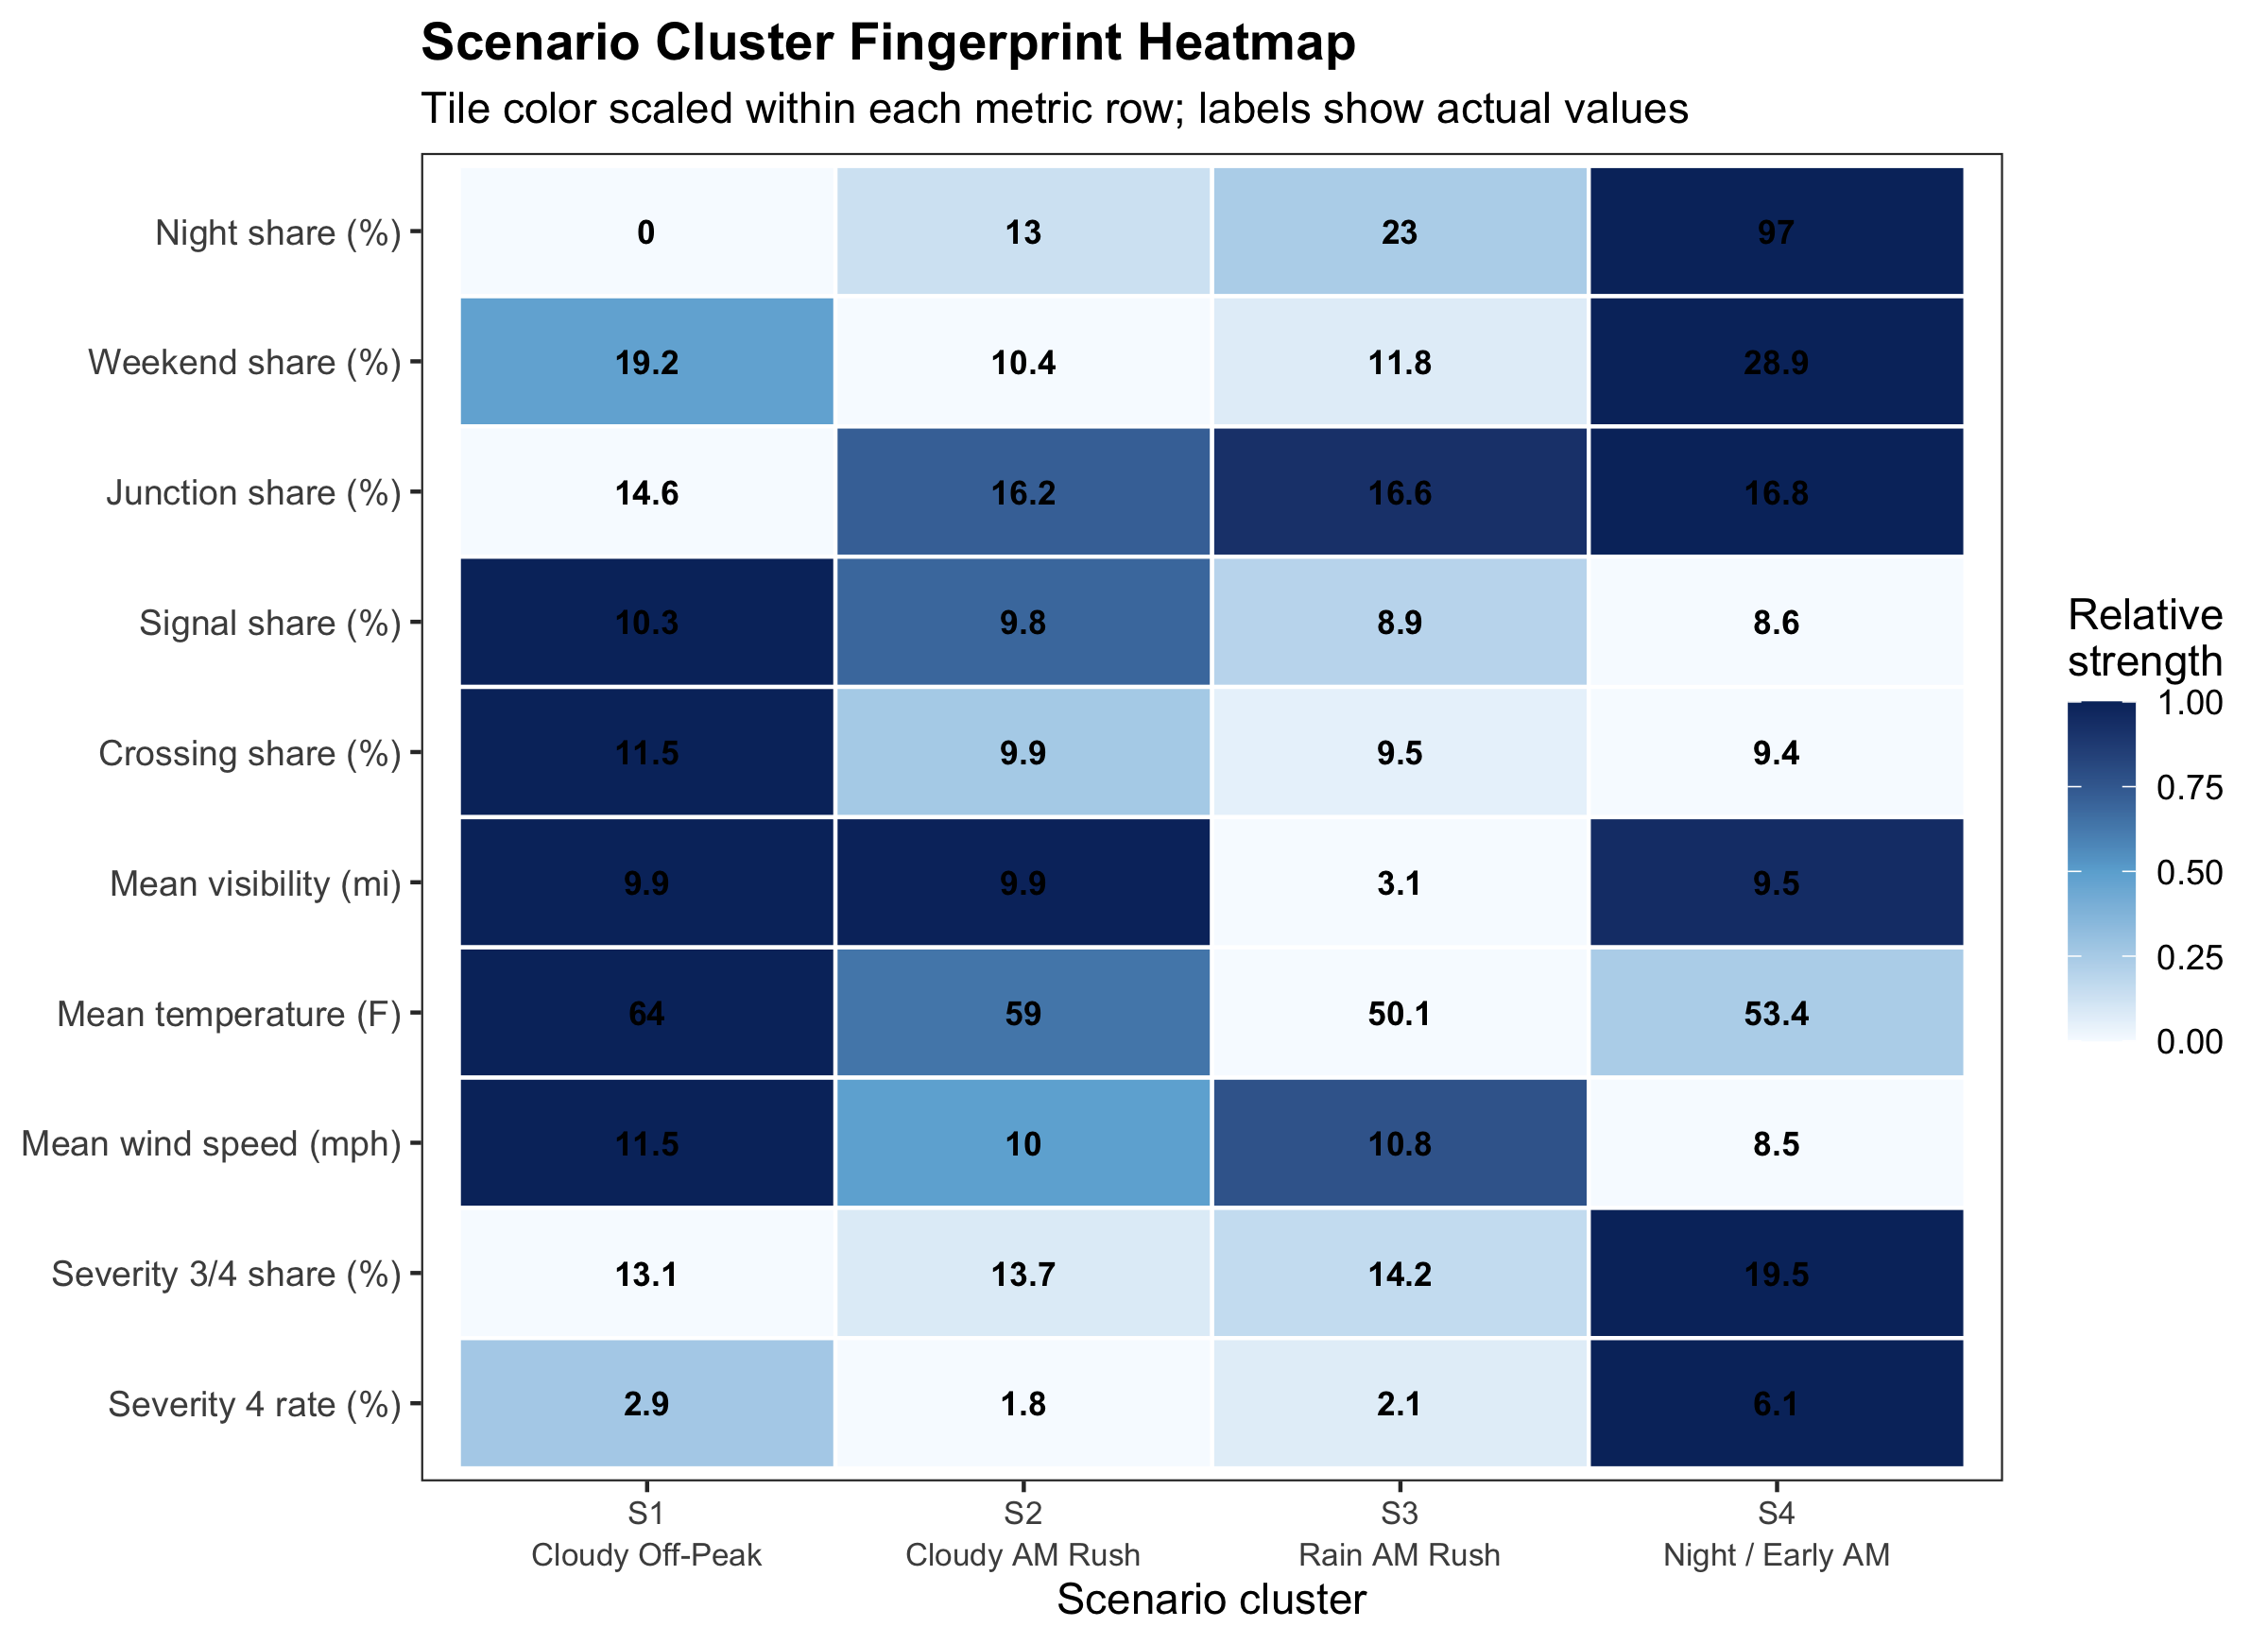
\includegraphics[width=0.70\textwidth]{figures/phase9_cluster_fingerprint_heatmap.png}
\caption{Standardised cluster fingerprints across all scenario features. Each column is a cluster; each row is a feature. The heatmap confirms visually distinct profiles for all four archetypes.}
\label{fig:fingerprint}
\end{figure}

%======================================================================
\section{Validation}
%======================================================================

\begin{table}[H]
\centering
\caption{Validation summary---all metrics against published thresholds.}
\begin{tabular}{@{}lccc@{}}
\toprule
\textbf{Metric} & \textbf{Score} & \textbf{Threshold} & \textbf{Verdict} \\
\midrule
Silhouette width & 0.4268 & $\geq$\,0.30 & \textbf{PASS} \\
Bootstrap ARI (20 reps) & 0.997 & $\geq$\,0.65 & \textbf{PASS} \\
ARI std.\ dev. & 0.0013 & --- & Near-perfect \\
RF classification accuracy & 99.6\% & --- & PASS \\
DBSCAN corridor count & 12 & 3--15 & PASS \\
DBSCAN noise fraction & 15.3\% & 5--30\% & PASS \\
Quality gate & \textsc{acceptable} & --- & \textbf{PASS} \\
\bottomrule
\end{tabular}
\end{table}

\begin{figure}[H]
\centering
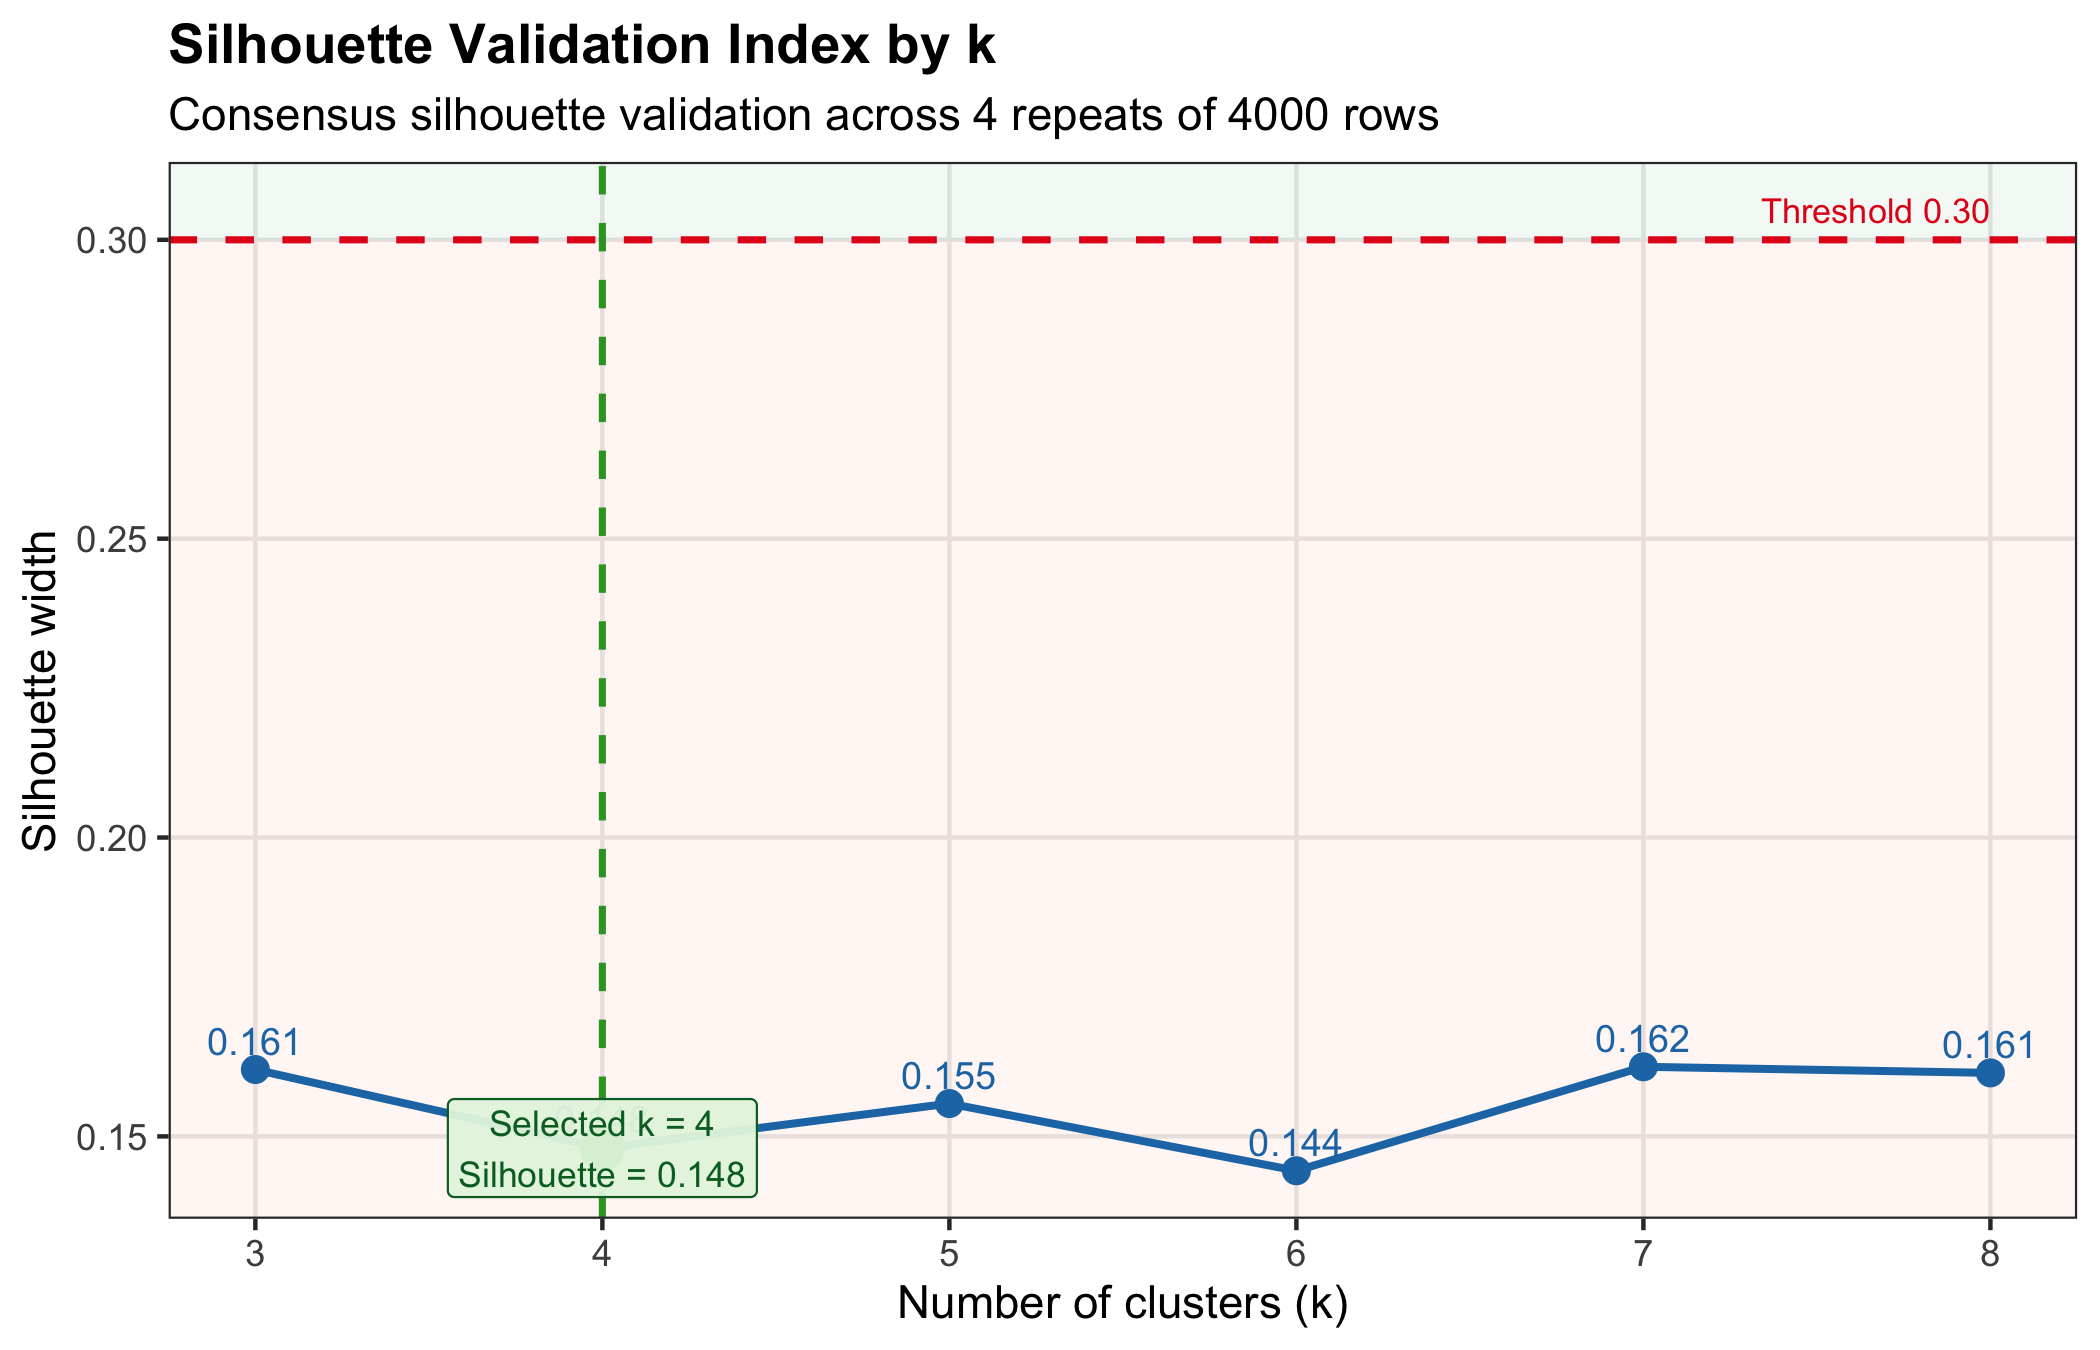
\includegraphics[width=0.58\textwidth]{figures/phase9_validation_index_plot.png}
\caption{Silhouette and within-cluster distance across candidate $k$ values.}
\label{fig:validation}
\end{figure}

%======================================================================
\section{Discussion}
%======================================================================

\subsection{Why FAMD Outperforms k-Prototypes}

The 165\% silhouette improvement stems from three reinforcing factors. First, feature selection removed 9 noise features that the Gower distance treated equally to informative ones. Second, FAMD's orthogonal projection concentrates discriminative variation into a few dimensions, whereas Gower averages across all original dimensions regardless of importance. Third, k-Means in Euclidean space benefits from well-established convergence guarantees that k-Prototypes with Gower distance does not share.

The 39.78\% variance retention might appear low, but it reflects a deliberate trade-off: the tail components describe within-cluster variation (e.g., minor temperature fluctuations) that is real but irrelevant for between-cluster separation. The grid search over (ncomp $\times$ k) provides empirical evidence that this trade-off is correct.

\subsection{Limitations}

\begin{itemize}[nosep]
\item \textbf{FAMD retains 39.8\% variance.} Four components were selected via grid search for optimal silhouette. This is a deliberate bias-variance trade-off, not information loss.
\item \textbf{Observational data.} All results describe associations, not causal relationships. Nighttime driving correlating with higher severity does not prove causation.
\item \textbf{Precipitation excluded} (20.1\% missing). An important weather signal is absent from the models.
\item \textbf{Severity~2 dominance} (85\%). Subtle differences among severe accident types may be masked by the large low-severity majority.
\item \textbf{DBSCAN corridor labels are heuristic.} Latitude-band assignments were not validated against authoritative highway shapefiles.
\end{itemize}

%======================================================================
\section{Community Applications}
%======================================================================

\subsection{Targeted Nighttime Safety Campaigns}

Cluster~4 (Night / Early~AM) accounts for 17\% of all accidents but 6.1\% Severity~4 rate---2.21$\times$ the baseline. The 29\% weekend share suggests recreational late-night driving contributes disproportionately. Targeted interventions along LIE and Northern/Southern State corridors during 10~PM--5~AM could include enhanced road lighting, dynamic speed advisories, and DUI checkpoint programmes.

\subsection{Infrastructure Prioritisation at AM-Rush Hotspots}

The AM Rush archetype (C2, 50\% of accidents) dominates 11 of 12 DBSCAN corridor clusters. While individually low-severity (1.8\% Sev4), the sheer volume makes this the costliest cluster in aggregate. Signal timing optimisation, congestion management, and junction redesign at the densest Northern/Southern State segments would reduce the largest source of daily disruption.

%======================================================================
\section{Conclusion}
%======================================================================

\begin{table}[H]
\centering
\caption{Research question summary.}
\begin{tabular}{@{}llll@{}}
\toprule
\textbf{Track} & \textbf{Method} & \textbf{Status} & \textbf{Key finding} \\
\midrule
Scenario & FAMD + k-Means, $k$=4 & \textsc{acceptable} & Night/Early AM cluster: 6.1\% Sev4 (2.21$\times$) \\
Spatial  & DBSCAN, eps=1.0\,km & \textsc{defensible} & 12 corridors; LIE, SSP, NSP confirmed \\
Explainability & RF + SHAP & \textsc{defensible} & rush\_hour is \#1 driver (importance 0.33) \\
\bottomrule
\end{tabular}
\end{table}

The FAMD dimensionality reduction strategy elevated scenario clustering from \textsc{exploratory} (silhouette 0.16, Jaccard 0.24) to \textsc{acceptable} (silhouette 0.43, ARI 0.997) by concentrating signal in four orthogonal components while removing nine noise features identified via SHAP importance analysis.
The central finding is that \emph{when} you drive is the dominant risk factor on Long Island, with nighttime driving producing more than double the baseline severe-accident rate.
Combined with DBSCAN's 12 corridor clusters and the Random Forest SHAP bridge, the pipeline provides an end-to-end, reproducible toolkit for data-driven traffic safety policy.

\end{document}
